\section{Aussagenlogik}

\begin{frame}
	\frametitle{Aussagenlogik}
	Aussagen sind Sätze, die entweder wahr oder falsch sind.\\
	Der Wahrheitswert muss dabei nicht unbedingt bekannt oder \enquote{tatsächlich ermittelbar} sein.
	
	\pause
	\begin{Beispiel}
		\begin{itemize}
			\item $ 1 + 1 = 2 $ ist eine Aussage. Sie ist wahr.
			\item \enquote{Es gibt nur endlich viele Primzahlen.} ist eine Aussage. Sie ist falsch.
			\pause
			\item Die Goldbachsche Vermutung ist eine Aussage. Ihr Wahrheitswert ist unbekannt.
			\pause
			\item Die Welt wird am 11.11.11111 untergehen ist auch eine Aussage. Wir werden ihren Wahrheitswert aber wohl niemals ermitteln können.
			\pause
			\item \enquote{Gelb} ist keine Aussage.
			\pause
			\item \enquote{Dieser Satz ist falsch.} ist keine Aussage. Dem Satz kann offensichtlich kein Wahrheitswert zugeordnet werden.
		\end{itemize}
	\end{Beispiel}
\end{frame}

\begin{frame}
	\frametitle{Zwei Grundsätze der Aussagenlogik}
	
	\begin{itemize}
		\pause
		\item Jede Aussage ist entweder falsch oder wahr.\\
		Wir schreiben im Folgenden $\BB= \{\text{w}, \text{f}\}$
		\pause
		\item Der Wahrheitswert einer zusammengesetzten Aussage ist durch die
		Wahrheitswerte der Teilaussagen eindeutig festgelegt. \\
		\enquote{$2 + 2 = 5 \; \bimp \; \text{Pinguine können fliegen}$} ist \textbf{wahr}.\\[0.2em]
		%TODO
		%Ex falso quodlibet
	\end{itemize}

	Wir abstrahieren daher vom Inhalt und betrachten \textbf{Aussagevariablen}.
\end{frame}

\begin{frame}
	\frametitle{Syntax}
	\begin{Definition}
		$Var_{AL}$ ist die Menge aller Aussagevariablen. \\
		$A_{AL} = \{ \bleftBr, \brightBr, \bnot, \bund, \boder, \bimp \} \cup Var_{AL}$
	\end{Definition}
	\pause
	\begin{Definition}
		$For_{AL}$ ist die Menge aller syntaktisch korrekten Formeln über $Var_{AL}$.\\
		Formal wird diese induktiv über Konstruktionsabbildungen definiert (\emph{VL}).
		Wendet man Klammereinsparungen an, entspricht das Ergebnis unserer intuitiven Verwendung.
	\end{Definition}
	\pause
	\begin{Beispiel}
		$$Var_{AL} = \{A, B, C\}$$
		$$For_{AL} = \{(A  \bimp B) \boder \bnot B, ...\}$$
	\end{Beispiel}
\end{frame}

\begin{frame}
	\frametitle{Semantik}
	Die Semantik einer aussagenlogischen Formel wird durch Auswertung bestimmt.\\
	Hierbei werden den Symbolen aus $A_{AL}$ boolsche Funktionen zugeordnet.
	
	\pause
	\begin{Definition}
		Eine \textbf{boolesche Funktion} ist eine Abbildung der Form
		$f: \BB^n \to \BB$.
	\end{Definition}

	\pause
	\begin{Beispiel}
		\enquote{Übliche} boolesche Funktionen sind  $b_{\bnot}$,
		$b_{\bund}$, $b_{\boder}$ und $b_{\bimp}$
	\end{Beispiel}
\end{frame}

\begin{frame}<handout:0>
	\frametitle{Semantik}
	\begin{center}
		\begin{huge}
			$$\only<1-2>{\boder}\only<3-4>{\bund}\only<5-6>{\bnot}\only<7-8>{\bimp}$$
		\end{huge}
		Wahrheitstabelle:
		\begin{table}
			\begin{tabular}{|c|c|c|}
				\hline 
				$A$ & \only<1-4,7-8>{$B$} & $\only<1-2>{A \boder B}\only<3-4>{A \bund B}\only<5-6>{\bnot A}\only<7-8>{A \bimp B}$ \\ \hline
				w & \only<1-4,7-8>{w} & \only<2>{w}\only<4>{w}\only<6>{f}\only<8>{w} \\ \hline
				w & \only<1-4,7-8>{f} & \only<2>{w}\only<4>{f}\only<6>{f}\only<8>{f} \\ \hline
				f & \only<1-4,7-8>{w} & \only<2>{w}\only<4>{f}\only<6>{w}\only<8>{w} \\ \hline
				f & \only<1-4,7-8>{f} & \only<2>{f}\only<4>{f}\only<6>{w}\only<8>{w} \\ \hline
			\end{tabular}
		\end{table}
	\end{center}
\end{frame}

\begin{frame}
	\frametitle{Semantik}
	Der Wahrheitswert einer zusammengesetzten Aussage hängt von den Wahrheitswerten der verwendeten Aussagevariablen ab. \\
	\begin{Definition}
		Sei $V \subseteq Var_{AL}$ die Menge der verwendeten Aussagevariablen.\\
		Eine Funktion $I: V \to \BB$ bezeichnet man als \textbf{Interpretation}.
	\end{Definition}
	
	\pause
	
	\begin{Definition}
		Eine \textbf{Tautologie} ist eine aussagenlogische Formel, bei der für alle möglichen Interpretationen $I$ gilt: $val_I(A) = \textbf{w}$.\\[0.5em]
		
		\pause
		Liefert die Auswertung von zwei aussagenlogischen Formeln $A$ und $B$ für jede Interpretation $I$ jeweils den gleichen Wert, also $val_I(A) = val_I(B)$, so bezeichnen wir diese Formeln als \textbf{äquivalent} und schreiben $A \equiv B$.
	\end{Definition}

\end{frame}

\begin{frame}
	\frametitle{Auswertung}
	Für die Auswertung einer Aussagenlogsichen Formel $A$ unter Interpretation $I$ definieren wir die Abbildung $val_I(A)$.\\
	Die Auswertung erfolgt dabei schrittweise.
	
	\begin{align*}
	&val_I((A \bimp B) \boder \bnot B)  \\
	\visible<2->{= \;&b_{\boder} (val_I(A\bimp B), val_I(\bnot B)) \\}
	\visible<3->{= \;&b_{\boder} (b_{\bimp} (val_I(A), val_I(B)), b_{\bnot}(val_I(B))) \\}
	\visible<4->{= \;&b_{\boder} (b_{\bimp} (I(A), I(B)), b_{\bnot}(I(B))) \\}
	\end{align*}
\end{frame}

% TODO
\begin{frame}
	\frametitle{Auswertung}
	\only<1|handout:1>{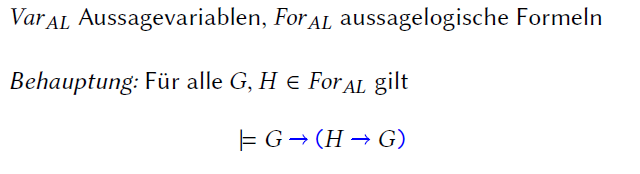
\includegraphics[scale=0.65]{al_uebung_1}\\[2em]
	Quelle: GBI-Übung 2015/2016}
	\only<2|handout:2>{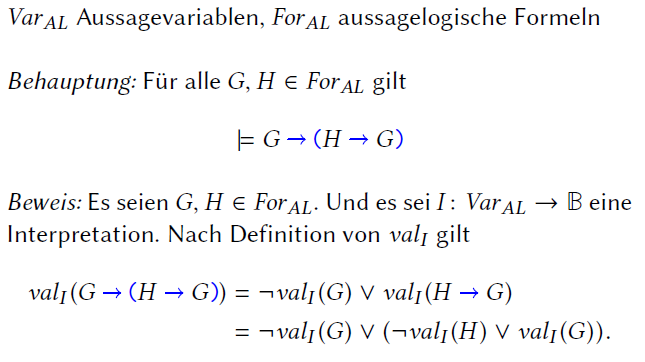
\includegraphics[scale=0.65]{al_uebung_2}}
	\only<3|handout:3>{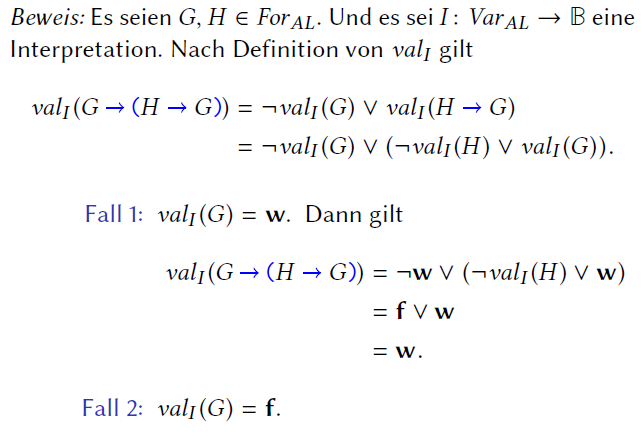
\includegraphics[scale=0.65]{al_uebung_3}}
	\only<4|handout:4>{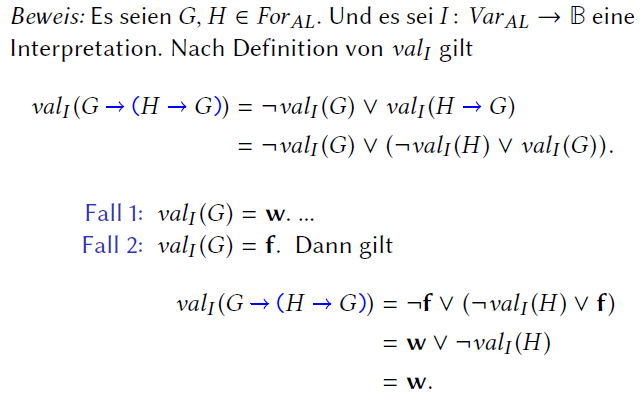
\includegraphics[scale=0.65]{al_uebung_4}}
	\only<5|handout:5>{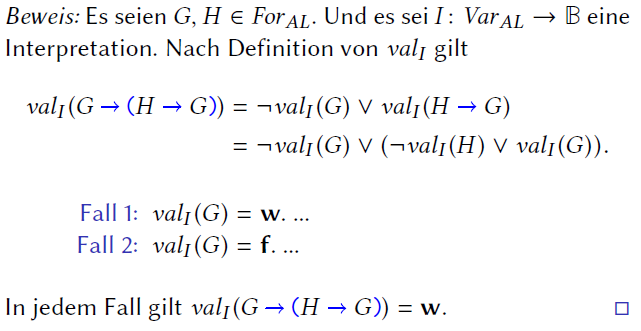
\includegraphics[scale=0.65]{al_uebung_5}}
\end{frame}

\begin{frame}
	\frametitle{Semantik}
	
	Möchte man eine AL-Formel für alle möglichen Interpretationen auswerten, so macht man dies meist in Form einer \textbf{Wahrheitstabelle}.
	
	\begin{block}{Aufgabe}
		Gegeben seien die Formeln
		$$ F_1 = (((B \bimp A) \boder B) \bimp (\bnot A)) \bund B$$
		und
		$$F_2 = \bnot A \bund B$$
		Stellen Sie die Wahrheitstabellen von $F_1$ und $F_2$ auf. Sind die beiden Formeln äquivalent?
	\end{block}
\end{frame}

\begin{frame}
	\frametitle{Lösung}
	Für die Formel $F_1$:
	\begin{table}[H]
	\centering
	\begin{tabular}{|*{6}{c|}}
	\hline
	$A$ & $B$ & $B \bimp A$ &  $\dots \boder B$ & $\dots \bimp \bnot A$ & $\dots \bund B$ \pause \\ \hline
	w & w & w & w & f & f \pause \\ \hline 
	w & f & w & w & f & f \pause \\ \hline
	f & w & f & w & w & w \pause \\ \hline
	f & f & w & w & w & f \\ \hline
	\end{tabular}
	\end{table}
\end{frame}

\begin{frame}
	\frametitle{Lösung}
	Für die Formel $F_2$:
	\begin{table}[h!]
	\centering
	\begin{tabular}{|*{3}{c|}}
	\hline
	$A$ & $B$ & $\bnot A \bund B$ \pause  \\ \hline
	w & w & f \pause  \\ \hline
	w & f & f \pause  \\ \hline
	f & w & w \pause  \\ \hline
	f & f & f \\ \hline
	\end{tabular}
	\end{table}
	Also sind die beiden Formeln äquivalent $$F_1 \equiv F_2$$
\end{frame}

\begin{frame}
	\frametitle{Beweisbarkeit}
	Kalkül, Axiome, Schlussregeln, Modus Ponens, ...\\
	Siehe VL!
\end{frame}